\documentclass[12pt, oneside]{article}
\usepackage{geometry} 
	\geometry{letterpaper, margin=1in}
\usepackage{graphicx}
\graphicspath{}
\usepackage{indentfirst}
\usepackage{subfig}
\usepackage{float}

%Package and setup for including nicely formatted and colored code in our report
\usepackage{listings}
\usepackage{color}

\definecolor{dkgreen}{rgb}{0,0.6,0}
\definecolor{gray}{rgb}{0.5,0.5,0.5}
\definecolor{mauve}{rgb}{0.58,0,0.82}

\lstset{frame=single,
  language=C,
  aboveskip=3mm,
  belowskip=3mm,
  showstringspaces=false,
  columns=flexible,
  basicstyle={\small\ttfamily},
  numbers=left,
  numberstyle=\tiny\color{gray},
  keywordstyle=\color{blue},
  commentstyle=\color{dkgreen},
  stringstyle=\color{mauve},
  breaklines=true,
  breakatwhitespace=true,
  tabsize=3
}

\title{ELE 381 Final Report: Who is the most influential artist on Spotify?}
\author{Akash Levy, Daniel Wood, Erica Wu, Sunny He, Vincent Po}
\date{\today}

% \setcounter{secnumdepth}{0} %Disable numbering

\begin{document}
\maketitle

\section{The Short Answer}

\section{The Long Answer}

\subsection{Motivation}
% Why we chose this topic, why/what spotify

\subsection{What is influence?}
% Also how do we plan on measuring it? (Methodology) Walkthrough maybe of scraping

\subsection{Setup}

\subsubsection{Data Collection Methodology}

\subsubsection{The Subgraph Boundary Problem}

\subsubsection{Directed vs. Undirected Networks}

\subsection{Results}

\subsubsection{Centrality}

\subsubsection{Page Rank}

\subsection{Observations of the Graph}

\subsubsection{Homophily}

\subsubsection{Cliques}

\subsection{Visualization Techniques}

\subsection{Final Summary}

\begin{figure}[H]
	\centering
	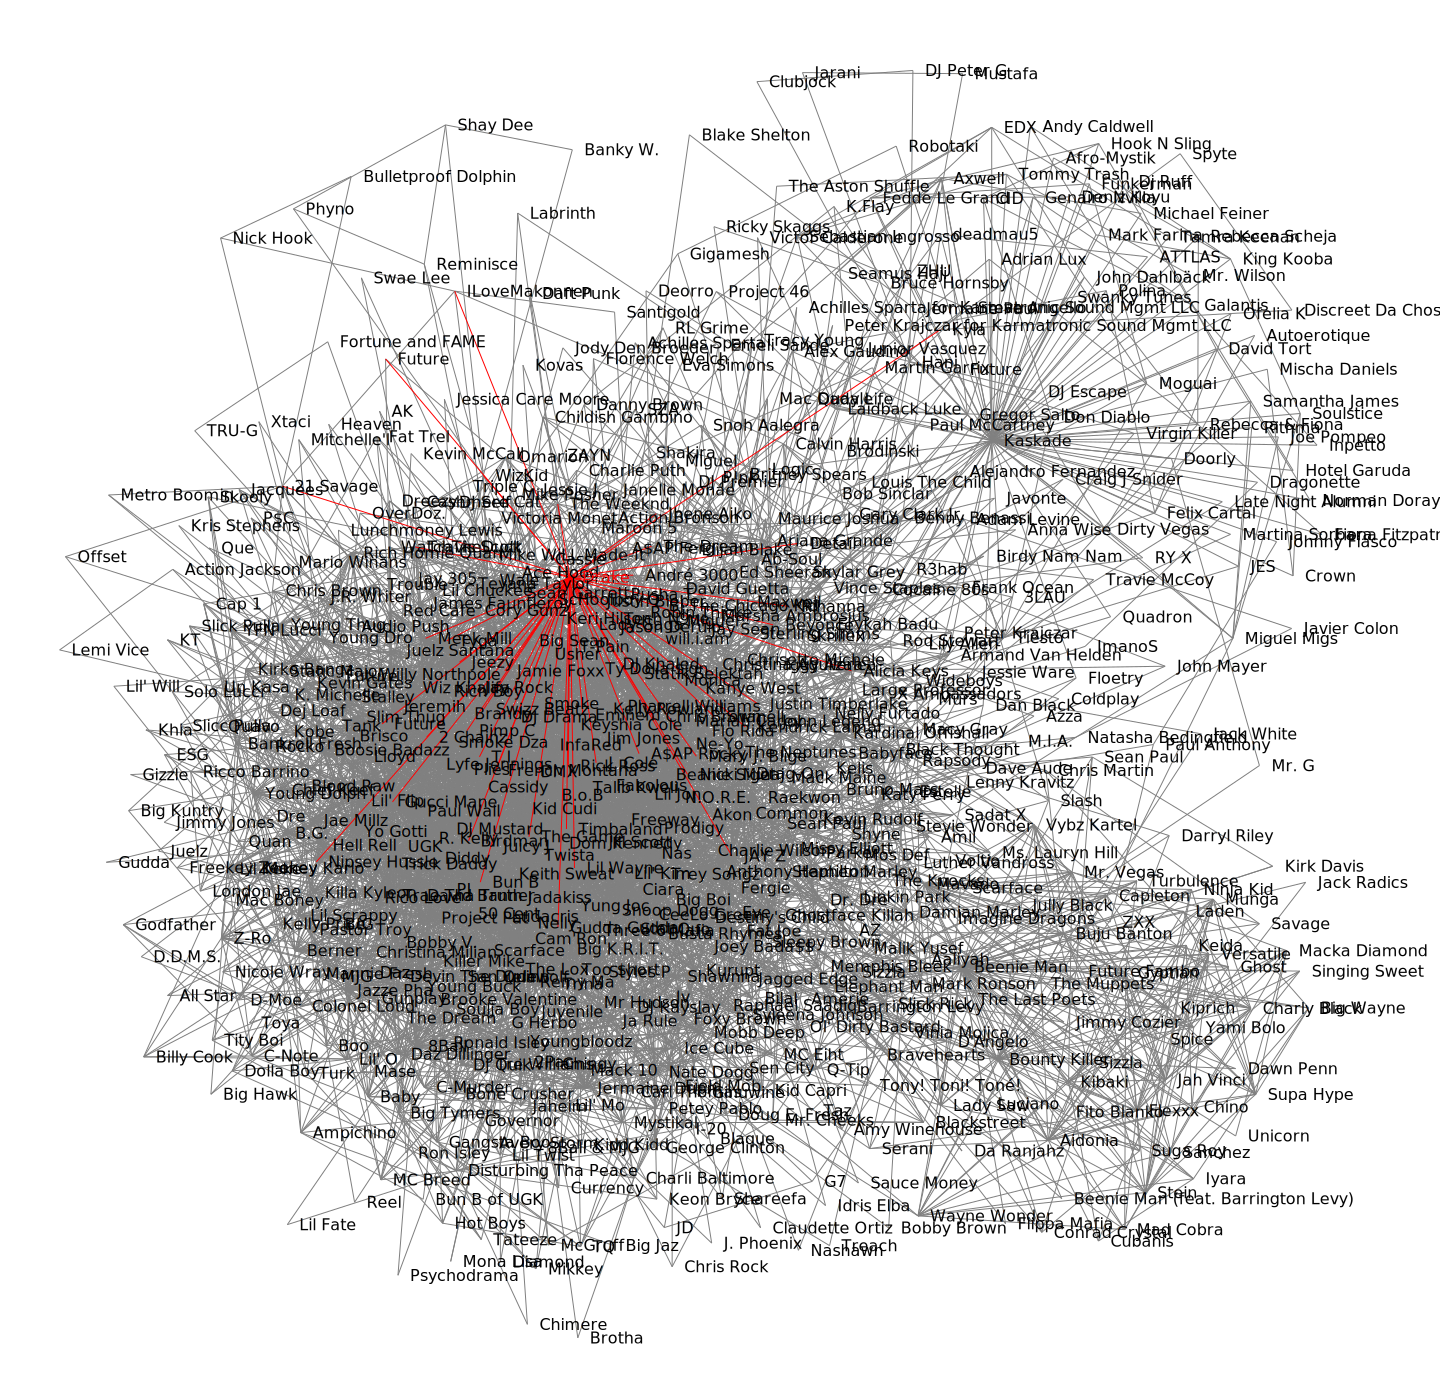
\includegraphics[width=0.5\textwidth]{./Pictures/graph4.png}
	\caption{Graph 4}
\end{figure}




% example for inserting graphs
%
%\begin{figure}[H]
%	\centering
%	\includegraphics[width=0.8\textwidth]{\Pictures\Analog.JPG}
%	\caption{Analog Circuitry Block Diagram}
%\end{figure}


\end{document}